\documentclass[Main]{subfiles}
\begin{document}

\chapter{Elicitation Process\fxnote{skal skrives færdig}}\label{cha:Elicitation}

This chapter describes the elicitation process carried out to create this requirement specification. 
In this chapter, "we" refers to the group of students carrying out the elicitation process.
\\

\begin{wrapfigure}{r}{0.6\textwidth}
\vspace{-20pt}
\begin{center}
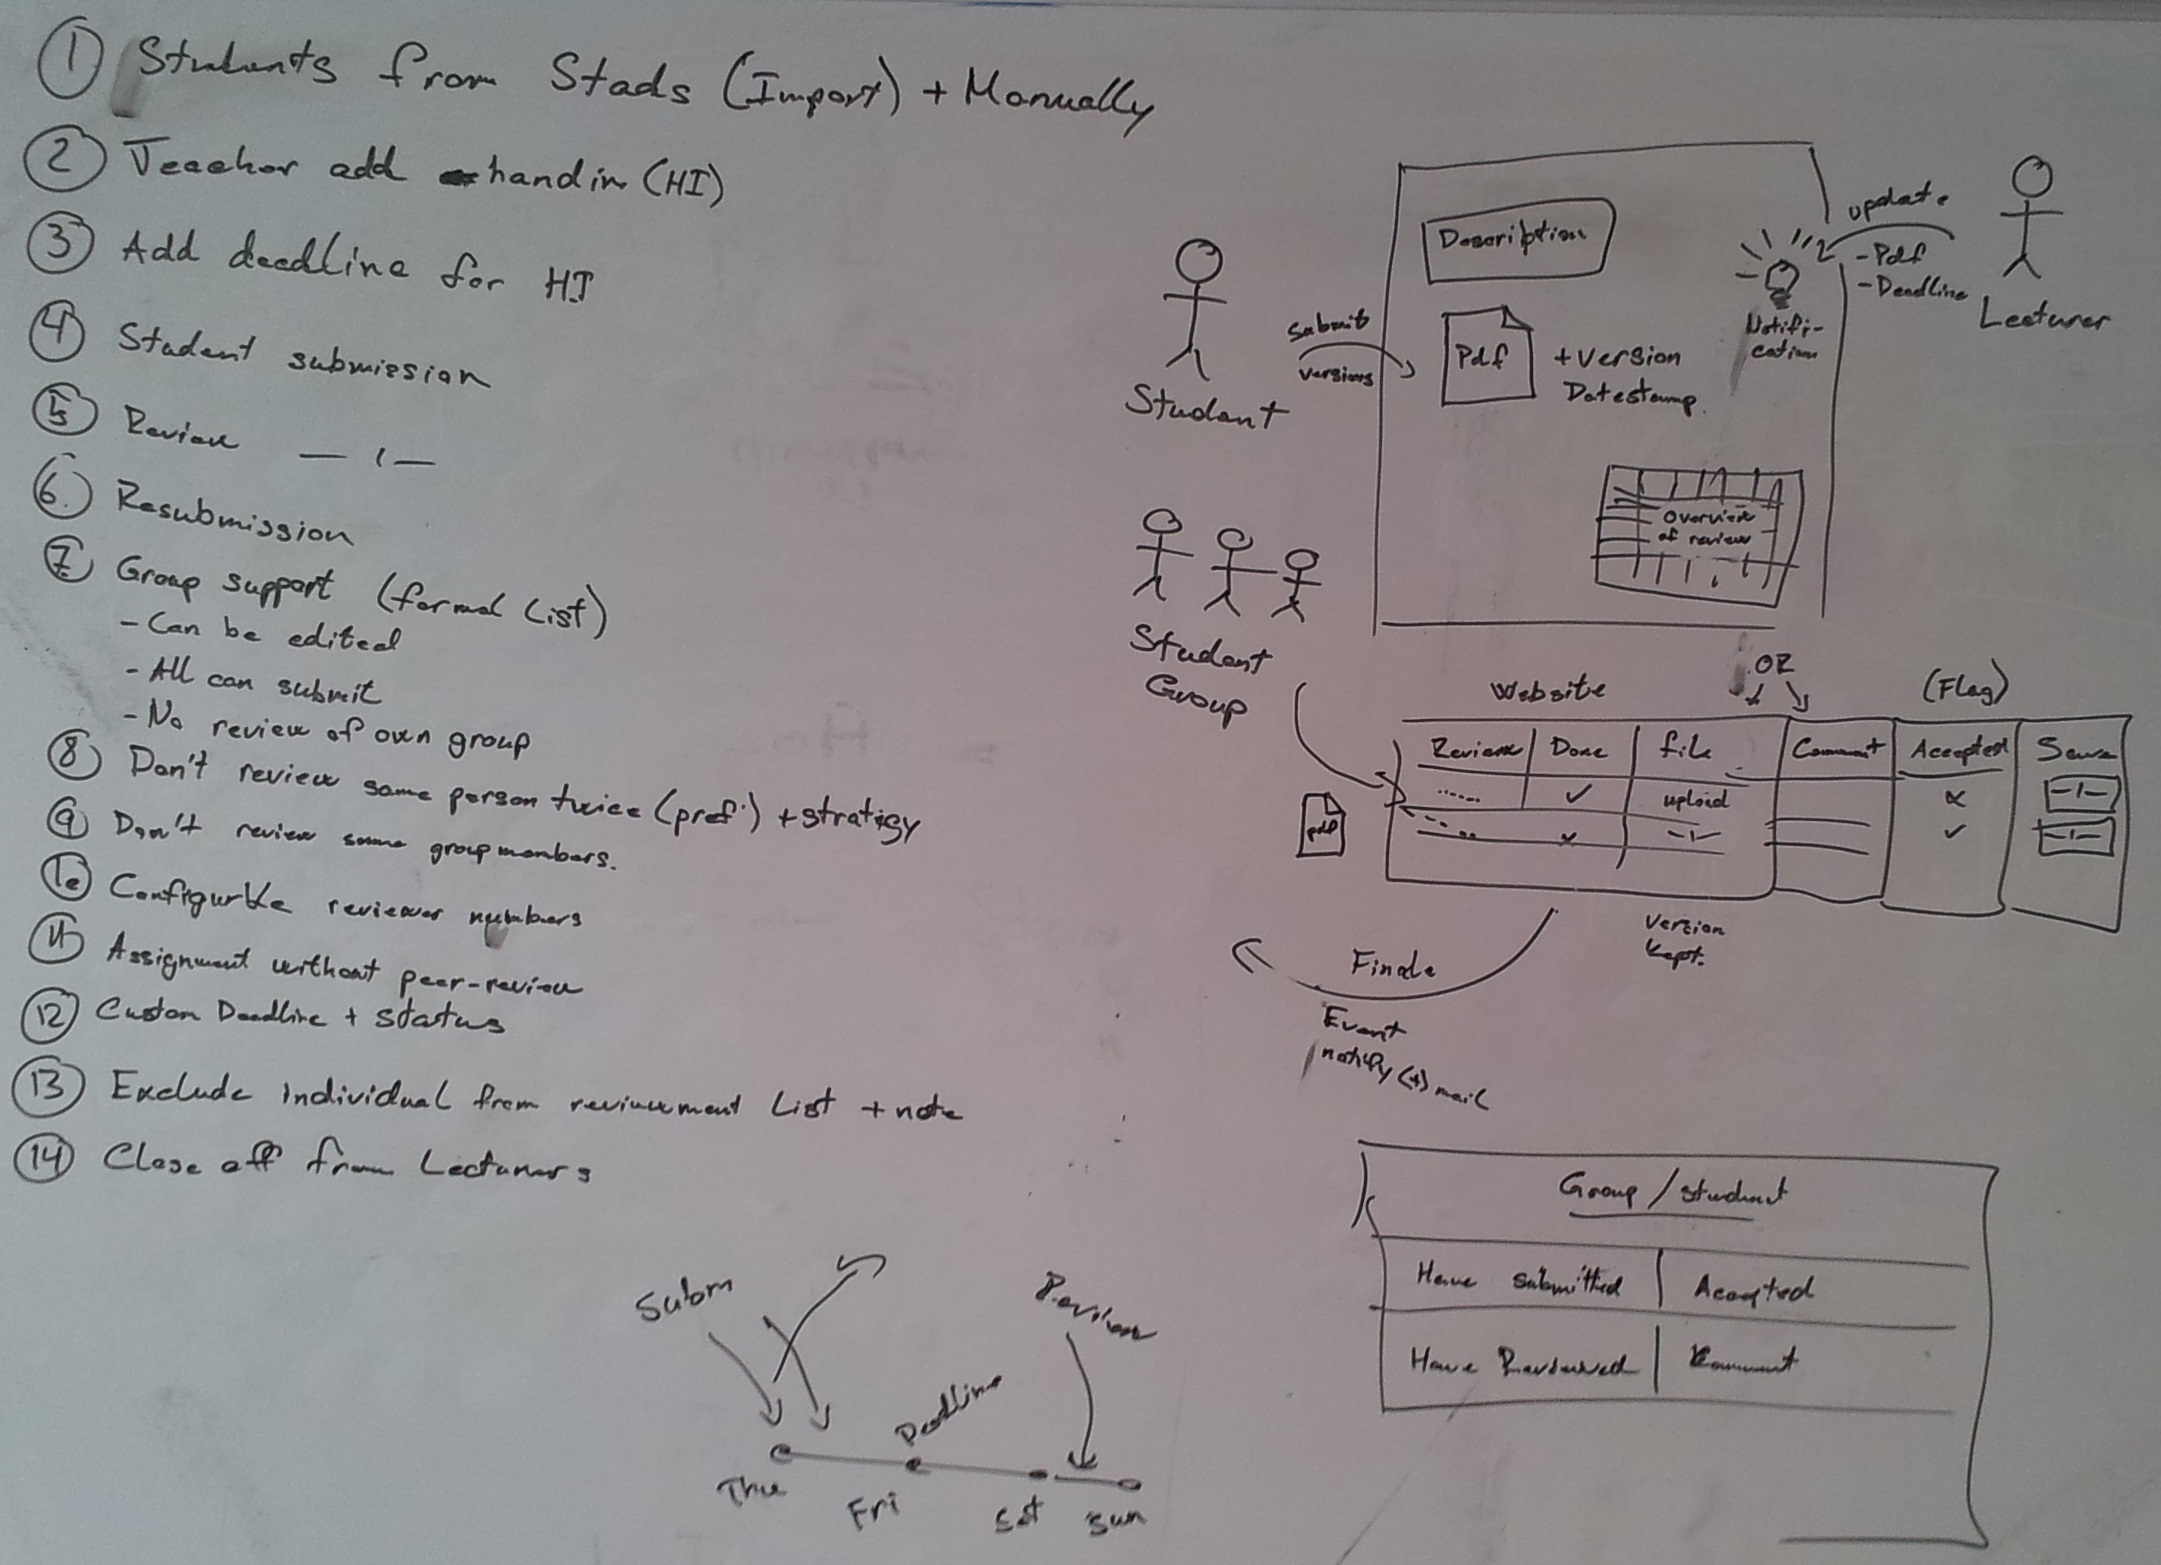
\includegraphics[width=0.58\textwidth]{IMG_20140221_131547.jpg}
\vspace{-5pt}
\end{center}
\vspace{-10pt}
\caption{Whiteboard notes created during user interview.}
\label{fig:UserInterviewNotes}
\vspace{-10pt}
\end{wrapfigure}

Before starting the elicitation process, the costumer provided a short description of the tasks this new system is intended to support. 
This description helped us gain an initial understanding of the costumer's business goals.
\\
\\
The system described by this requirement specification is intended to be used by lecturers and students during the ITDMAT course. 
While not part of the elicitation process per se, we participated in said course, thus allowing us to observe the work process as users. 
Observing the work process contributed to our domain knowledge, by being exposed to the issues and problems of the current situation.
\\
\\
To get an understanding of what the customer actually needed user interviews were conducted with the costumer. 
\\
\\
Not used:
\begin{itemize}
\item Questionnaires -- Was outside the scope of this project.
\item Brainstorm -- New ideas was not needed.
\item Domain workshop -- Not needed. The system was well-understood.
\item Focus group
\item Stakeholder analysis(implicit) -- Finding the goal of the customer helped understand the system.
\end{itemize}

The above is normal procedures to follow when making an SRS which also is the reason only 2 meetings with the customer was held.
On the first meeting we brought tasks and system events written in small notes and presented the system for the customer.
Since we had a clear idea of the troubles the course had without a system, we had a lot of suggestions for features the system could provide for both the lecture and the student.
Many of these where agreeable for the customer who had had similar ideas but not written them down in the user description. 
At the same meeting a few things needed visualization, as seen on Figure \ref{fig:UserInterviewNotes}, showing how users of the system can interact with the system and what responses they can expect.

The second meeting was with a draft of the SRS, which quickly revealed a clear mistake is a section, but also showed us how easy it is to find and understand tasks in the document.



\end{document}